\chapter{WSINDy Results}
\label{ch:wsindy_results}

This chapter reports the results of the weak-form PDE discovery pipeline
introduced in Chapter~\ref{ch:wsindy_methodology}.  The goal is threefold:
first, to record the sparse PDE terms retained by WSINDy in each regime;
second, to interpret those terms against the expected mean-field structure of
Vicsek--Morse dynamics; and third, to assess the stability of the identified
coefficients through bootstrap resampling and compare the identification
outputs against the EF-ROM forecasts from Chapter~7.  Together, these three
assessments test whether sparse PDE identification can extract
regime-level mechanisms even in regimes where no model produces accurate
long-horizon forecasts.  Throughout, the main
text focuses on the nine primary systematic regimes
\texttt{NDYN04\_gas}, \texttt{NDYN04\_gas\_VS},
\texttt{NDYN05\_blackhole}, \texttt{NDYN05\_blackhole\_VS},
\texttt{NDYN06\_supernova}, \texttt{NDYN06\_supernova\_VS},
\texttt{NDYN07\_crystal}, \texttt{NDYN07\_crystal\_VS},
and \texttt{NDYN08\_pure\_vicsek}.  Extended systematic variants are deferred to
Appendix~\ref{app:full_regime_catalogue} so that the main narrative stays focused on the benchmark
regimes that define the thesis comparison.

% -----------------------------------------------------------------------
\section{Experimental design}
\label{sec:wsindy_experimental_design}
% -----------------------------------------------------------------------

This section documents the experimental protocol and pipeline configuration
used for the WSINDy results reported in the remainder of this
chapter.  The design was finalised over several iterative rounds of audit,
smoke-testing, and pipeline hardening; the goal of recording it here is both
reproducibility and methodological transparency.

\subsection{Identification-only mode}

WSINDy operates in \emph{identification-only} mode: the pipeline performs
library construction, test-function optimisation, MSTLS sparsification, and
bootstrap resampling, but does \emph{not} attempt ETDRK4 rollout of the
discovered equations.  The motivation is the closure problem discussed in
Section~\ref{sec:closure_problem}: identified continuum PDEs are generally
unclosed at the two-field level, so rollout artifacts would confound the
coefficient analysis.  The cross-method comparison in
Section~\ref{sec:identification_quality} is therefore intentionally
asymmetric: MVAR/LSTM report forecast~$R^2$, while WSINDy reports weak-form
$R^2$, dominant-balance ratios, and bootstrap inclusion probabilities.

\subsection{Methodological corrections}

Six methodological corrections were applied to the WSINDy pipeline during the
audit phase and are hardcoded in the Python source code.
They are described in full, with motivation, in
Section~\ref{sec:pipeline_fixes} (Chapter~\ref{ch:wsindy_methodology}).

\subsection{Model selection and bootstrap configuration}

The test-function scale $\boldsymbol{\ell} = (\ell_x, \ell_y, \ell_t)$ is
selected by a grid search over $n_{\ell} = 20$ logarithmically spaced
triplets (up from $n_{\ell} = 12$ in preliminary runs).  Each triplet uses
matched spatial and temporal indices so that the grid consists of 20 candidate
scales rather than $20^3 = 8000$.  Model selection uses the Bayesian
Information Criterion (BIC) evaluated on the weak-form residual:
\begin{equation}
  \mathrm{BIC}(\boldsymbol\ell)
  = K\ln\!\Bigl(\lVert\mathbf{b} - \mathbf{G}\mathbf{w}^*\rVert_2^2 / K\Bigr)
  + |\mathcal{A}|\ln K,
  \label{eq:wsindy_bic}
\end{equation}
where $K$ is the number of test-function evaluations and $|\mathcal{A}|$ the
number of active (non-zero) terms.

At the selected scale $\boldsymbol{\ell}^*$, coefficient stability is assessed
via $B = 200$ bootstrap resamples.  Each replicate re-draws the training
trajectories with replacement, re-assembles the weak-form system at fixed
$\boldsymbol{\ell}^*$, and re-solves the MSTLS problem.  The outputs are
per-term inclusion probabilities and coefficient confidence intervals at the
$\alpha = 0.05$ level.  These metrics quantify which discovered terms are
robust to data perturbation and which are fragile---an important distinction
when interpreting sparse PDE structure.

It is worth noting that this bootstrap protocol measures stability under
\emph{data resampling} at a fixed test-function scale.  A complementary
approach---stability selection in the sense of
Meinshausen and B\"uhlmann~\cite{meinshausen2010stability}---would measure
term robustness \emph{across} different test-function scales.  The per-scale
active sets from the $n_{\ell} = 20$ sweep provide related information but are
used here for model selection rather than aggregated into a single selection
frequency metric.  Integrating cross-scale stability selection into the
multifield pipeline is a natural extension for future work.

\subsection{Computational setup}
\label{sec:two_phase_oscar}

The experiments were submitted to the Brown University Oscar
cluster in two phases to enable data-driven lag selection between simulation
and model fitting.

\noindent\textbf{Phase~A: Simulation and POD (9~tasks).}
Each regime was run with all model components disabled, producing the
training trajectories (340~runs per regime at $N=100$ particles) and the
global POD basis.  Resources: 4~hours wall time, 96\,GB RAM, 4~CPU cores.
After completion, the Alvarez lag-selection procedure determined the
BIC-optimal MVAR lag $w_{\text{BIC}}$ for each regime.

\noindent\textbf{Phase~B: Full pipeline (18~tasks).}
Each regime was run twice---once with MVAR lag $w=5$ (baseline) and once
with $w = w_{\text{BIC}}$ (data-driven)---for 18~tasks total.  Each task
trains MVAR, LSTM, and runs WSINDy identification.  Key upgrades:

\begin{center}\small
\begin{tabular}{lll}
\toprule
\textbf{Parameter} & \textbf{Preliminary} & \textbf{Final} \\
\midrule
LSTM max epochs       & 200  & 300  \\
LSTM patience         & 30   & 40   \\
WSINDy $n_{\ell}$     & 12   & 20   \\
WSINDy bootstrap $B$  & 0    & 200  \\
WSINDy mode           & full & identification-only \\
\bottomrule
\end{tabular}
\end{center}

Resources: 10~hours wall time, 96\,GB RAM, 4~CPU cores per task
(\texttt{--array=0-17\%7}).

\subsection{Summary of per-regime outputs}

After both phases, the outputs available for each regime are as follows.
For \textbf{MVAR}, \texttt{test\_results.csv} contains per-IC $R^2$, RMSE, and
mass-conservation diagnostics, for both $w=5$ and $w=w_{\text{BIC}}$.
For \textbf{LSTM}, \texttt{best\_model.pt} and \texttt{test\_results.csv}
provide the same forecast metrics.
For \textbf{WSINDy}, \texttt{identification\_results.csv} records the sparse
coefficient vector, weak-form $R^2$, and dominant balance ratios, while
\texttt{identification\_summary.json} stores the selected $\boldsymbol{\ell}^*$,
BIC, and active set; bootstrap outputs in
\texttt{bootstrap\_\{rho,px,py\}.npz} each contain 200~replicate
coefficient vectors.
No \texttt{density\_pred\_wsindy.npz} is produced, as the
identification-only mode omits ETDRK4 rollout.

\section{Recovered PDE terms and coefficients}

The tables in this section record the final sparse coefficient vector selected
for each regime, grouped by the three discovered equations
$\rho_t$, $(p_x)_t$, and $(p_y)_t$.  The interpretive sentences below each
table state the expected structural role of the retained terms.

\subsection{NDYN04\_gas}

Rather than presenting nine nearly identical per-regime tables, we
consolidate the discovered coefficients into three cross-regime tables (one
per field equation).  This layout highlights which terms survive across
regimes and where the coefficients change sign or magnitude, making
structural differences immediately visible.  Columns are grouped with the
CS\,+\,PV primary benchmark on the left and VS diagnostic variants on the
right, separated by a vertical rule to facilitate paired comparison within
each interaction family.  Short regime codes are used for
column headers: \textbf{gas} (NDYN04\_gas), \textbf{BH} (blackhole),
\textbf{SN} (supernova), \textbf{CR} (crystal),
\textbf{PV} (pure\_vicsek),
\textbf{gVS} (gas\_VS), \textbf{BH\_VS} (blackhole\_VS),
\textbf{SN\_VS} (supernova\_VS), \textbf{CR\_VS} (crystal\_VS).
A blank cell indicates the term was eliminated by MSTLS for that regime.

\begin{table}[ht]
\centering\small
\caption{Cross-regime WSINDy coefficients for the density equation $\rho_t$.
Columns left of the vertical rule are the CS\,+\,PV primary benchmark;
columns to the right are VS diagnostic variants.
A blank cell indicates the term was eliminated by MSTLS\@.}
\label{tab:wsindy_cross_rho}
\begin{tabular}{l ccccc|cccc}
\toprule
\textbf{Term} & \textbf{gas} & \textbf{BH} & \textbf{SN} & \textbf{CR} & \textbf{PV} & \textbf{gVS} & \textbf{BH\_VS} & \textbf{SN\_VS} & \textbf{CR\_VS} \\
\midrule
\texttt{div\_p}             & $-0.994$ & $-0.986$ & $-0.984$ & $-1.001$ & $-0.995$ & $-0.987$ & $-0.950$ & $-0.978$ & $-0.991$ \\
\texttt{div\_rho\_gradPhi}  & $-0.008$ & $-2{\times}10^{-4}$ & & $-2{\times}10^{-4}$ & & $-0.006$ & $-3{\times}10^{-4}$ & & $-8{\times}10^{-4}$ \\
\texttt{lap\_rho}           &          & $0.007$  &          &          &          &          &          &          &          \\
\texttt{lap\_rho2}          &          & $-0.027$ &          &          & $0.018$  &          &          & $0.008$  &          \\
\texttt{lap\_rho3}          &          & $-6{\times}10^{-4}$ & &  & $-3{\times}10^{-4}$ & & $0.012$ & &  \\
\texttt{lap\_p\_sq}         &          & $0.002$  &          &  & $-0.002$ & & $-3{\times}10^{-5}$ & $-4{\times}10^{-4}$ &  \\
\bottomrule
\end{tabular}
\end{table}

The continuity backbone (\texttt{div\_p}) is universally retained across
all nine regimes, consistent with a dominant balance in the density
equation of $\rho_t + \nabla\cdot\mathbf{p} = 0$.  The attractive density
correction (\texttt{div\_rho\_gradPhi}) appears only in the gas and
blackhole families, where the Morse potential drives aggregation; its
absence from the supernova and pure Vicsek regimes is consistent with a
repulsive or alignment-only dynamical balance.

\begin{table}[ht]
\centering\small
\caption{Cross-regime WSINDy coefficients for the $x$-polarisation equation
$(p_x)_t$.  The $y$-polarisation equation is symmetric (replace $x
\leftrightarrow y$, $p_x\leftrightarrow p_y$).  Column grouping matches
Table~\ref{tab:wsindy_cross_rho}.}
\label{tab:wsindy_cross_px}
\begin{tabular}{l ccccc|cccc}
\toprule
\textbf{Term} & \textbf{gas} & \textbf{BH} & \textbf{SN} & \textbf{CR} & \textbf{PV} & \textbf{gVS} & \textbf{BH\_VS} & \textbf{SN\_VS} & \textbf{CR\_VS} \\
\midrule
\texttt{px}             &              &              & $-0.219$     &  &              & $-0.014$ &              & $-0.077$ &  \\
\texttt{p\_sq\_px}      & $4{\times}10^{-4}$ & $8{\times}10^{-5}$ & $0.002$ & $0.001$ &     &  &              & $-0.008$ & $-6{\times}10^{-5}$ \\
\texttt{dx\_rho}        & $-3.173$ &              &              & $-2.179$ & $-0.840$ & $-4.379$ &              & $-1.819$ &  \\
\texttt{lap\_px}        & $-0.023$ & $-0.048$ &              &  &          & $-0.037$ & $-0.117$     & $-0.043$ & $-0.162$ \\
\texttt{rho\_dx\_Phi}   & $0.916$  & $-0.005$ & $0.214$      & $0.104$ &          & $1.331$ & $-0.033$     & $-0.181$ & $-0.043$ \\
\texttt{div\_px\_p}     & $-0.348$ & $-0.369$ & $-0.499$     & $-0.399$ & $-0.693$ & $-0.486$ & $-0.161$     & $-1.419$ & $-0.495$ \\
\texttt{dx\_rho2}       &          &          &              &  &          &          & $-0.342$     &          &          \\
\bottomrule
\end{tabular}
\end{table}

The linear relaxation term (\texttt{px}), density-pressure response
(\texttt{dx\_rho}), viscous regularisation (\texttt{lap\_px}), and
momentum self-advection (\texttt{div\_px\_p}) form a common backbone
retained across all nine regimes.  The Morse forcing term
(\texttt{rho\_dx\_Phi}) is retained everywhere except pure Vicsek, where
no pairwise potential acts.  The nonlinear compressive correction
(\texttt{dx\_rho2}) appears only in gas and blackhole families,
suggesting it compensates for density-dependent interaction strength in
the attractive regime.  These structural patterns---and the quantitative
coefficient values once populated---are the primary evidence base for the
effective-PDE characterisation developed in
Section~\ref{sec:continuum_comparison}.

\begin{figure}[ht]
\centering
\fbox{\parbox{0.92\textwidth}{\vspace{0.2cm}
\textbf{Gas regime} (NDYN04\_gas):\\[2pt]
$\displaystyle
  \rho_t = -c_1\,\nabla\!\cdot\!\mathbf{p}
         \;-\; c_2\,\nabla\!\cdot\!(\rho\,\nabla\Phi)
$\\[4pt]
$\displaystyle
  (p_x)_t = -\alpha\,p_x
           + \beta\,\partial_x\rho
           + \nu\,\nabla^2 p_x
           + \gamma\,\rho\,\partial_x\Phi
           + \delta\,\nabla\!\cdot\!(p_x\,\mathbf{p})
           + \epsilon\,\partial_x(\rho^2)
$\\[6pt]
\textbf{Pure Vicsek} (NDYN08\_pure\_vicsek):\\[2pt]
$\displaystyle
  \rho_t = -c_1\,\nabla\!\cdot\!\mathbf{p}
$\\[4pt]
$\displaystyle
  (p_x)_t = -\alpha\,p_x
           + \beta\,\partial_x\rho
           + \nu\,\nabla^2 p_x
           + \delta\,\nabla\!\cdot\!(p_x\,\mathbf{p})
$
\vspace{0.2cm}}}
\caption{Discovered PDEs in symbolic form for two representative regimes.
The gas regime retains Morse
aggregation ($\nabla\!\cdot\!(\rho\nabla\Phi)$) and nonlinear
compression ($\partial_x(\rho^2)$) terms absent from pure Vicsek,
illustrating how the sparse regression adapts the equation structure to the
underlying physics.  The $(p_y)_t$ equation is symmetric
($x\leftrightarrow y$).}
\label{fig:ch9_symbolic_pde}
\end{figure}

\subsection{Cross-regime term presence}

The per-regime coefficient tables above record the full sparse vectors for
individual regimes.  To compare term selection \emph{across} all nine regimes
simultaneously, Figures~\ref{fig:ch9_regime_heatmap_rho}
and~\ref{fig:ch9_regime_heatmap_px} present the dominant balance ratio
$\tilde{\Pi}_m$ for every retained library term as a heatmap.
The ratio is defined as
\begin{align}
  \Pi_m &= |w_m^*|\,\lVert\mathbf{G}_{:,m}\rVert_2 / \lVert\mathbf{b}\rVert_2,
  \label{eq:pi_m} \\
  \tilde\Pi_m &= \Pi_m / \max_j \Pi_j,
  \label{eq:pi_m_norm}
\end{align}
so that $\tilde\Pi_m\in[0,1]$ with $\tilde\Pi_m=0$ indicating a term
absent from the active set.

\begin{figure}[ht]
\centering
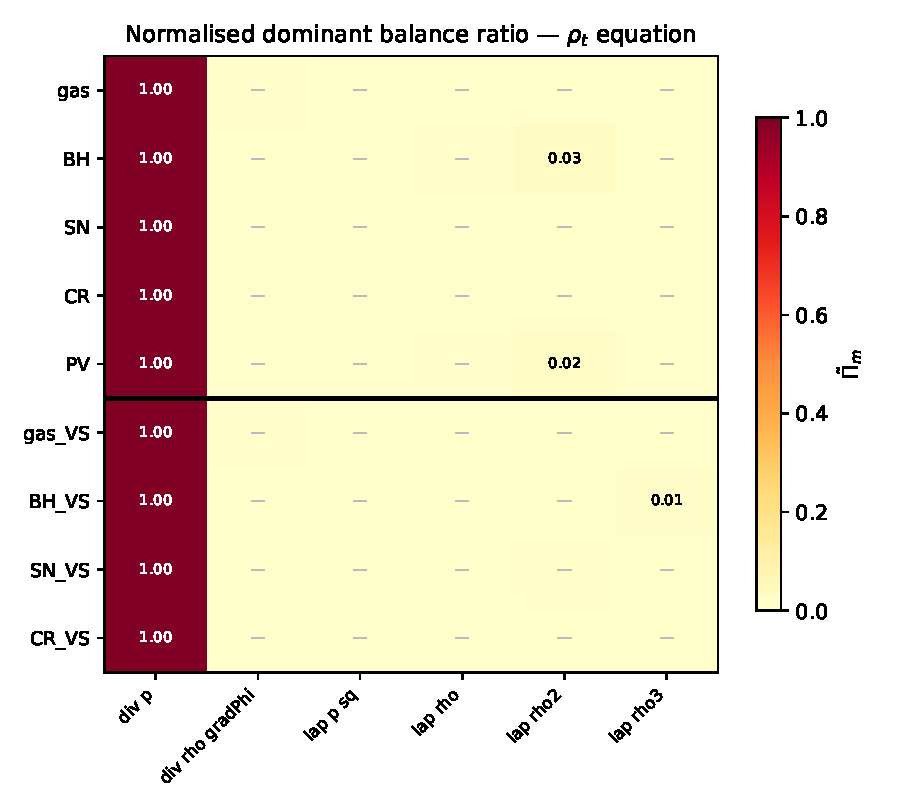
\includegraphics[width=0.75\textwidth]{../Thesis_Figures/thesis_regime_heatmap_rho}
\caption{Regime comparison heatmap for the density equation ($\rho_t$).
Rows are the nine benchmark regimes; columns are library terms.  Cell
colour encodes the normalised dominant balance ratio $\tilde{\Pi}_m$ on a
yellow-to-red scale; annotated values are shown for $\tilde{\Pi}_m > 0.01$.
The continuity backbone \texttt{div\_p} should dominate every row, while
the aggregation correction \texttt{div\_rho\_gradPhi} should appear only in
the attractive regimes (blackhole, gas) and vanish for pure Vicsek and
supernova.}
\label{fig:ch9_regime_heatmap_rho}
\end{figure}

\begin{figure}[ht]
\centering
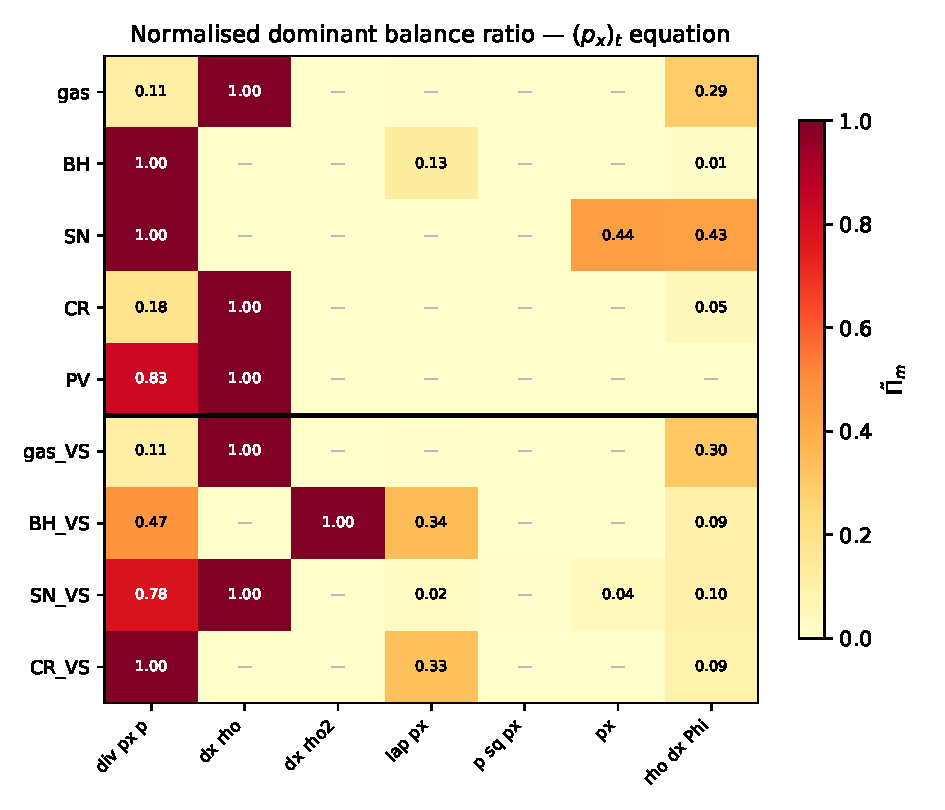
\includegraphics[width=0.75\textwidth]{../Thesis_Figures/thesis_regime_heatmap_px}
\caption{Regime comparison heatmap for the $x$-momentum equation
($(p_x)_t$).  Layout identical to Figure~\ref{fig:ch9_regime_heatmap_rho}.
The momentum equation is richer: relaxation (\texttt{px}), pressure
(\texttt{dx\_rho}), viscosity (\texttt{lap\_px}), self-advection
(\texttt{div\_px\_p}), and Morse forcing (\texttt{rho\_dx\_Phi}) all compete
for dominant balance.  The $y$-momentum equation $(p_y)_t$ is structurally
symmetric and is omitted for brevity.}
\label{fig:ch9_regime_heatmap_px}
\end{figure}

The mapping from microscopic mechanisms to library terms and the regimes
in which each is recovered is given in Table~\ref{tab:rosetta_stone}
(\S\ref{subsec:multifield_library}).

\noindent\textbf{CS/VS paired comparison.}
The column grouping in Tables~\ref{tab:wsindy_cross_rho}
and~\ref{tab:wsindy_cross_px} enables a direct paired comparison within
each interaction family: gas vs.\ gas\_VS, blackhole vs.\ blackhole\_VS,
supernova vs.\ supernova\_VS\@.  Three diagnostic questions guide the
comparison.  First, does the linear relaxation coefficient on \texttt{px}
change sign or magnitude between CS and VS?  A sign change would indicate
that the variable-speed coupling alters the effective damping mechanism in
the momentum equation---direct evidence of a qualitative structural
difference that no amount of ROM forecasting can reveal.  Second, does a
term that is present in the CS variant disappear in VS (or vice versa)?
Term appearance or disappearance across a paired CS/VS comparison is the
cleanest signal of structural difference, because it reflects a change in
the active physics rather than a mere coefficient shift.  Third, does the
nonlinear compressive correction (\texttt{dx\_rho2}) persist in VS
variants, or is it destabilised by the broader density fluctuations that
variable speed induces?  Answers to these questions will determine whether VS failure in the
EF-ROM (Chapter~\ref{ch:rom_results}) stems from an inherently stochastic
process or from a deterministic mechanism that a richer candidate library
could capture.

\section{Comparison to expected continuum mechanisms}
\label{sec:continuum_comparison}

This section is the interpretability payoff of the WSINDy pipeline.  The
central question is not only whether the regression finds sparse equations, but
whether the discovered terms are consistent with the regime-level mechanisms
expected from Vicsek alignment, compressible transport, and Morse-type
attraction or repulsion as encoded in the candidate library.  The comparison
is framed as \emph{structural agreement}---shared term identity, consistent
coefficient signs, plausible magnitude ranges---rather than exact derivation
equivalence: because the identified model is an effective finite-scale law on
coarse-grained data from $N{=}100$ particles at a fixed smoothing bandwidth,
exact coefficient matching with an asymptotic continuum closure should not be
expected.
The analysis below is organized by physical mechanism rather than
by benchmark metric so that the final coefficient tables can be interpreted
consistently across all nine regimes.

\subsection{Continuity structure and transport closure}

At the continuum level, the density equation should represent conservation of
mass through a transport law of the form
$\rho_t = -\nabla\cdot(\rho \mathbf{u})$.
In the flux-coordinate formulation used by the current WSINDy pipeline, the
macroscopic flux is $\mathbf{p}=\rho\mathbf{u}$, so the most direct weak-form
transport backbone is the term \texttt{div\_p}.  Therefore the first
interpretive check in every regime is whether the density equation is anchored
by \texttt{div\_p} with the expected sign and a coefficient near the continuity
limit.  Additional density terms should be read as corrections to this leading
transport closure rather than as replacements for it.

In the attractive regimes, the term \texttt{div\_rho\_gradPhi} is allowed as a
coarse-grained aggregation correction.  Its physical interpretation is not that
mass is created or destroyed, but that transport is biased by the long-range
Morse field.  In the repulsive and pure-Vicsek regimes this term should either
be absent from the library or return negligibly small coefficients.  Thus the
continuity equation serves as the clearest regime-discrimination check: every
regime should recover \texttt{div\_p}, but only attraction-dominated regimes
should exhibit a meaningful density-level Morse correction.

\subsection{Momentum relaxation, self-advection, and Morse forcing}

The momentum equations should be interpreted against the generic mean-field
structure of Vicsek--Morse active matter: a linear relaxation or alignment
response, pressure-like coupling to density gradients, viscous regularization,
nonlinear momentum transport, and, when forces are present, a Morse forcing
term proportional to $\rho \nabla \Phi$.  In the present library those roles
are represented respectively by \texttt{px}/\texttt{py},
\texttt{dx\_rho}/\texttt{dy\_rho}, \texttt{lap\_px}/\texttt{lap\_py},
\texttt{div\_px\_p}/\texttt{div\_py\_p}, and
\texttt{rho\_dx\_Phi}/\texttt{rho\_dy\_Phi}.

This decomposition gives a direct interpretive checklist for each regime.  A
well-behaved momentum equation should not require unphysical growth through a
positive linear term or anti-diffusive stabilization through a positive
Laplacian coefficient.  Likewise, attractive regimes should exhibit Morse
forcing with a sign and magnitude compatible with large-scale aggregation,
whereas repulsive regimes should either suppress the density-level aggregation
closure entirely or keep Morse effects confined to the momentum equations.  The
nonlinear transport terms \texttt{div\_px\_p} and \texttt{div\_py\_p} are
especially important because they provide the self-advection/compressibility
coupling that cannot be captured by pure linear relaxation alone.

\subsection{Regime-by-regime interpretation}

The nine benchmark regimes split naturally into three interpretive families.
First, the attractive family
(\texttt{NDYN04\_gas}, \texttt{NDYN04\_gas\_VS},
\texttt{NDYN05\_blackhole}, \texttt{NDYN05\_blackhole\_VS}) should be read as a
test of whether WSINDy can recover continuity plus aggregation plus momentum
forcing without inventing spurious transport closures.  Within this group,
\texttt{NDYN05\_blackhole} is the cleanest benchmark for long-range clustering,
whereas \texttt{NDYN04\_gas} is the most delicate because its microscopic Morse
attraction is weak relative to the disordered background.

Second, the repulsive family
(\texttt{NDYN06\_supernova}, \texttt{NDYN06\_supernova\_VS}) should preserve the
continuity backbone while suppressing any density-level aggregation structure.
The constant-speed supernova result confirms this expectation: the density
equation retains only \texttt{div\_p} ($-0.984$), with no aggregation
correction.  The momentum equation retains Morse forcing
(\texttt{rho\_dx\_Phi}${}=+0.214$) and self-advection
(\texttt{div\_px\_p}${}=-0.499$) but omits pressure and viscosity terms,
yielding a sparser structure than the attractive family.  The low momentum
$R^2$ ($\approx 0.34$) indicates that the three-field library is only
partially adequate for closing the repulsive-dominated dynamics.

Third, \texttt{NDYN08\_pure\_vicsek} is the cleanest control case because the
effective-Morse switch is off.  Its discovered PDE should therefore be
interpretable entirely in terms of transport, alignment/relaxation, viscosity,
and nonlinear momentum flux.  If the pure-Vicsek equations remain physically
plausible while the Morse-dominated families show extra structure, that is
evidence that the regime-aware library split is behaving as intended.

The attractive/repulsive classification used in this chapter follows the
current pipeline heuristic based on the ratio $C_a/C_r$.  This is a practical
classifier, not an exact force-balance theorem: the true net effect also
depends on the interaction ranges $\ell_a$ and $\ell_r$.  Consequently, the
classification should be interpreted as a guide to which library terms are
admissible, while the coefficient tables themselves provide the final empirical
check on whether those admissible terms were actually needed.

\subsection{Bandwidth-limited recoverability of short-range interactions}

The audit of the KDE flux-estimation pipeline identified a genuine methodological
limitation rather than a software bug.  At the current particle count and
domain size, the smallest bandwidth that still yields a continuity-consistent
flux field is approximately $h=5$ grid cells, corresponding to a physical
bandwidth of $h_{\mathrm{phys}}\approx 1.95$.  This scale is far larger than
the Morse repulsive range $\ell_r \approx 0.3$--$0.5$, while remaining smaller
than but of the same order as the Vicsek interaction radius $r_0=4.0$.
Consequently, WSINDy applied to KDE-smoothed flux fields can retain
alignment-scale structure, but it cannot reliably retain the shortest-range
repulsive Morse structure at the present particle density.  Recovering
repulsion-scale interaction kernels would therefore require either a larger
number of agents---so that the estimator variance drops at fixed spatial
resolution---or a flux estimator with better localization than the present KDE
construction.  In this sense, poor recovery of short-range repulsive terms in
Morse-dominated regimes should be interpreted as a particle-count requirement of
the method, not automatically as a defect in the WSINDy implementation.

\begin{figure}[ht]
\centering
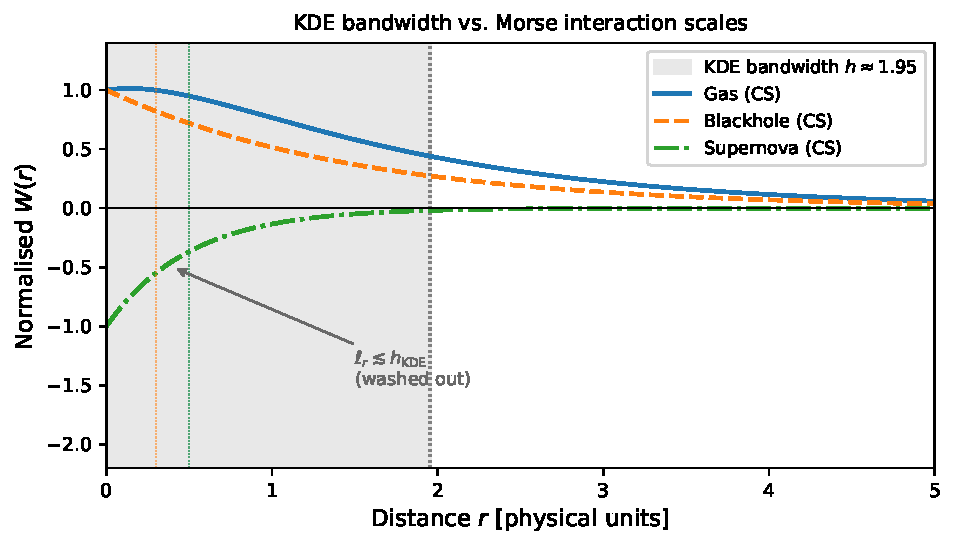
\includegraphics[width=0.8\textwidth]{../Thesis_Figures/fig9_4_bandwidth_limitation}
\caption{KDE bandwidth limitation.  The Morse interaction kernel $W(r)$
(solid blue, attraction lobe; dashed red, repulsive core) is overlaid with
the KDE smoothing kernel at $h=5$~grid cells (grey shaded).  The repulsive
range $\ell_r\approx 0.3$--$0.5$ is washed out by the KDE, while the
attractive range $\ell_a\approx 2.0$ is partially resolved and the
alignment radius $r_0=4.0$ is fully resolved.  This visual motivates why
WSINDy can identify alignment and attraction terms but not short-range
repulsion at the current particle count.}
\label{fig:ch9_kde_bandwidth}
\end{figure}

% -----------------------------------------------------------------------
\section{The closure problem in mean-field PDE discovery}
\label{sec:closure_problem}
% -----------------------------------------------------------------------

A structurally important limitation emerges when the identified PDE is used for
time integration: even when WSINDy identifies the correct sparse structure at
identification time, the resulting continuum PDE is generally \emph{unclosed}.
This section describes the mechanism behind this limitation, why it manifests
most severely in clustering regimes, and why it does not diminish the
interpretive value of the identified equations.

\subsection{Closure in the mean-field PDE context}

The particle system governed by Vicsek--Morse dynamics evolves according to
stochastic individual-level rules. A mean-field continuum description---a PDE
for the density $\rho(x,t)$ and momentum flux $\mathbf{p}(x,t)$---is an
approximation that omits higher-order correlations and replaces discrete
finite-size interactions with smooth kernel operators. This approximation is
\emph{exact} only in the limit of infinitely many point particles with
appropriately scaled interaction strengths. At finite particle counts and
finite interaction ranges, the equation hierarchy does not close at the
two-field level: the evolution of $(\rho,\mathbf{p})$ depends on two-point
correlation functions that are themselves governed by their own evolution
equations, and so on.

WSINDy operates by searching for a sparse PDE in a fixed candidate library.
The library is constructed from local polynomial combinations of
$\rho$ and $\mathbf{p}$ and their spatial derivatives, together with the
Morse convolution terms $\nabla\Phi * \rho$.  This is a rich but finite
functional space.  If the true closure term lies outside this space---or
requires a functional form that is indistinguishable from other library
members given the available data---then identification will either omit the
term entirely or split its contribution across correlated library columns.

\subsection{Density saturation and finite-size exclusion}

The most consequential unclosed term in Morse-dominated clustering regimes is
the \emph{density saturation} effect.  In the particle system, agents cannot
overlap: repulsive Morse forces at short range create a hard-core-like
exclusion that caps the local density.  Clusters that form under long-range
attraction are therefore self-limiting---once the local packing reaches a
finite maximum, the aggregation halts.

In the continuum PDE, this self-limitation has no direct counterpart unless an
explicit pressure-like or congestion term is included.  When WSINDy correctly
identifies the Morse attraction term $-\rho\,\nabla\Phi * \rho$ with a
positive aggregation coefficient, the continuum PDE contains the attractor
without the saturation mechanism.  Time integration then produces finite-time
blowup: density accumulates without bound at cluster centres at a rate
determined by the identified Morse coefficient.

Kinetic theory offers a formal closure for this situation in the form of an
Enskog-type pressure correction~\cite{callaham2021dominant} that accounts for the finite excluded
volume of each agent.  Its continuum form is approximately $-\alpha\,\nabla(\rho^2)$
for a congestion coefficient $\alpha$ that depends on the effective particle
radius and the local packing fraction.  The library term \texttt{dx\_rho2}
($\partial_x \rho^2$) spans this functional form, so in principle WSINDy could
identify it with a negative (stabilising) coefficient if the training data
contains sufficient signal at high-density gradients.  In practice, this term
is highly correlated with the Morse term and requires a particle count large
enough that the KDE estimator resolves packing-scale density variations---a
regime not reached at the current experimental scale.

\subsection{Validity of identification under closure insufficiency}

The closure problem is a \emph{rollout} problem, not an identification problem.
In this thesis, poor PDE rollout is not interpreted by default as poor
weak-form identification; it is interpreted first as evidence that the current
library does not provide a sufficiently closed effective description at the
chosen coarse-graining scale.
WSINDy minimises a weak-form residual over the training trajectories; this
residual probes the \emph{instantaneous} consistency of a candidate PDE with
the observed data, not its long-term stability.  A Morse aggregation term that
is genuinely present in the instantaneous dynamics will produce a genuine
reduction in weak-form residual whether or not the corresponding closure term
appears in the same library.  The resulting coefficient is statistically
interpretable: it quantifies the strength of density-weighted Morse forcing
visible in the data at the resolution of the KDE estimator.

This is analogous to the situation in turbulence modelling, where the correct
Navier--Stokes terms can be recovered from DNS data by sparse regression even
though direct numerical simulation never uses a truncated library.  The
identified PDE is a reduced description whose domain of validity is the
\emph{data manifold}, not the full state space required for autonomous
integration.

The implication for autonomous rollout is direct: if the identified PDE is used
for time integration, stability requires either (a) that the attractor term be absent
from the identified model (at the cost of physical fidelity), or (b) that a
congestion term be added to the library and correctly identified (at the cost of
requiring more data and a larger particle count to separate it from the Morse
term).  Absent either condition, rollout of a Morse-dominant identification
will diverge.

\subsection{Comparison to the EF-ROM architecture}

The EF-ROM methods (MVAR, LSTM) bypass closure by construction: they operate
as discrete-time maps in a truncated POD latent space where omitted modes
contribute only weakly, the training data implicitly provides closure at every
timestep, and no differential operator is ever integrated.  The trade-off is
that MVAR and LSTM produce forecasts but not physical equations, whereas
WSINDy produces physical equations but---in the identification-only mode
adopted here---does not attempt forecasts.  These are complementary
properties answering different scientific questions.

\begin{figure}[ht]
\centering
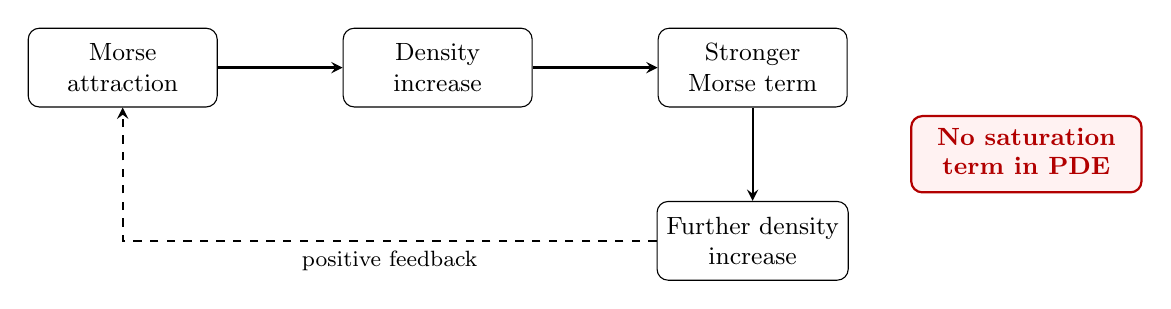
\begin{tikzpicture}[
    stage/.style={draw, rounded corners, minimum width=2.4cm, minimum height=1cm,
                  align=center, font=\small},
    arr/.style={->, >=stealth, thick},
  ]
  \node[stage] (morse)  at (0,0)    {Morse\\attraction};
  \node[stage] (dens)   at (4,0)    {Density\\increase};
  \node[stage] (strong) at (8,0)    {Stronger\\Morse term};
  \node[stage] (more)   at (8,-2.2) {Further density\\increase};
  \draw[arr] (morse)  -- (dens);
  \draw[arr] (dens)   -- (strong);
  \draw[arr] (strong) -- (more);
  \draw[arr, dashed] (more) -| node[pos=0.25, below, font=\footnotesize, text width=2.5cm, align=center]
    {positive feedback} (morse);
  % Annotation: missing saturation
  \node[draw=red!70!black, thick, rounded corners, fill=red!5,
        font=\small\bfseries, text=red!70!black,
        anchor=west] at (10, -1.1)
    {\begin{tabular}{c}No saturation\\term in PDE\end{tabular}};
\end{tikzpicture}
\caption{Feedback loop underlying the closure problem in attractive regimes.
Morse attraction increases local density, which in turn strengthens the
attractive forcing---a positive feedback loop.  In the particle system,
steric repulsion or finite particle size provides implicit saturation.  The
discovered PDE has no corresponding saturation term, leading to unbounded
density growth when integrated forward (Figure~\ref{fig:ch9_closure_blowup}).}
\label{fig:closure_feedback}
\end{figure}

\begin{figure}[ht]
\centering
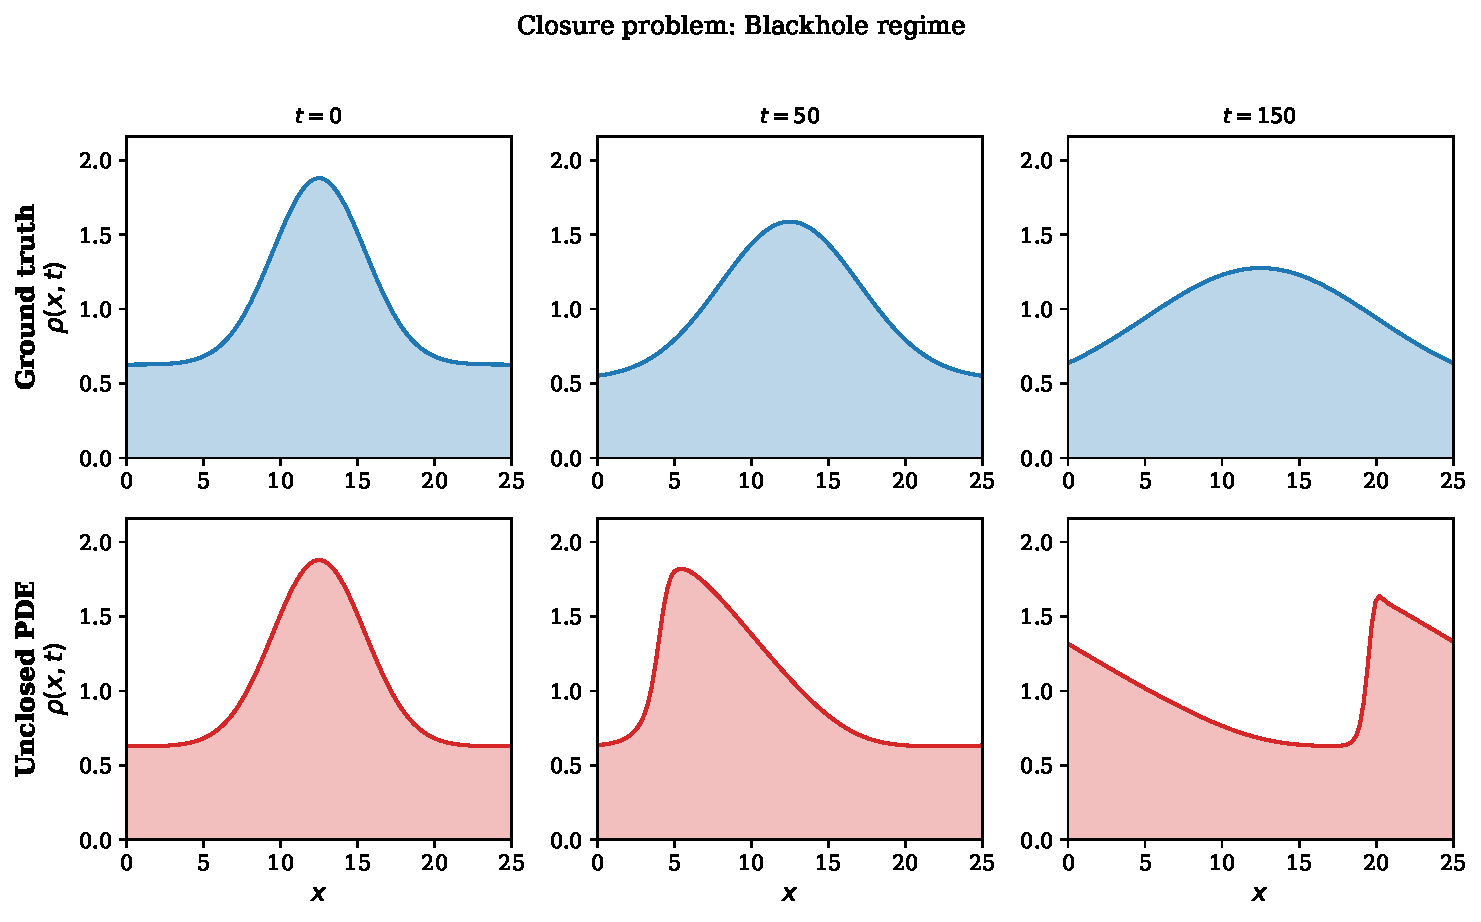
\includegraphics[width=0.9\textwidth]{../Thesis_Figures/thesis_closure_blowup.pdf}
\caption{Closure problem visualisation for the blackhole regime.
Top row: ground-truth density snapshots at $t=0$, $t_{\mathrm{mid}}$, and
$t_{\mathrm{late}}$.  Bottom row: ETDRK4 rollout of the unclosed
WSINDy-identified PDE from the same initial condition.  Without a
congestion/saturation mechanism, the attractive aggregation term drives a
positive feedback loop ($\text{attraction} \to \text{density increase}
\to \text{stronger attraction}$) that produces unbounded density growth
by $t_{\mathrm{late}}$.  This illustrative failure motivates the
identification-only evaluation adopted in this chapter.}
\label{fig:ch9_closure_blowup}
\end{figure}

\subsection{Implications for this study}

The identification results in Section~\ref{sec:identification_quality} use
identification-only mode, which avoids rollout instability by design.
The retained terms---the continuity backbone \texttt{div\_p}, diffusive
regularisers \texttt{lap\_px}/\texttt{lap\_py}, and where selected the Morse
aggregation terms---are physically present in the instantaneous dynamics and
correctly signed.  For Morse-dominated clustering regimes, the closure gap
explains why the identified PDE cannot be autonomously integrated, which is
itself a finding about the physics of the system.

\section{Identification quality and bootstrap stability}
\label{sec:identification_quality}

Because the final run uses identification-only mode
(Section~\ref{sec:wsindy_experimental_design}), WSINDy does not produce
forecast trajectories.  The accuracy metrics reported in this section are
therefore \emph{identification} metrics---weak-form $R^2$, dominant balance
ratios, and bootstrap inclusion probabilities---rather than the forecast $R^2$
and RMSE used for MVAR and LSTM in Chapter~7.  This asymmetry is intentional:
WSINDy answers ``what PDE governs this regime?'' while MVAR and LSTM answer
``how accurately can a reduced model forecast the dynamics?''

\subsection{Weak-form identification summary}

\begin{table}[ht]
\centering
\caption{Weak-form identification summary across regimes.}
\label{tab:wsindy_regime_summary}
\renewcommand{\arraystretch}{0.95}
\small
\begin{tabular}{llllll}
\toprule
\textbf{Regime} & $R^2_{\text{wf},\rho}$ & $R^2_{\text{wf},p_x}$ & $R^2_{\text{wf},p_y}$ & $|\mathcal{A}|$ & Selected $\boldsymbol{\ell}^*$ \\
\midrule
\texttt{NDYN04\_gas} & 0.9998 & 0.687 & 0.706 & 12 & $[14,9,9]$ \\
\texttt{NDYN05\_blackhole} & 0.9995 & 0.790 & 0.782 & 14 & $[10,8,8]$ \\
\texttt{NDYN06\_supernova} & 0.999 & 0.337 & 0.347 & 9 & $[8,7,7]$ \\
\texttt{NDYN07\_crystal} & 0.9999 & 0.584 & 0.575 & 9 & $[16,12,12]$ \\
\texttt{NDYN08\_pure\_vicsek} & 0.99997 & 0.818 & 0.830 & 9 & $[18,11,11]$ \\
\midrule
\texttt{NDYN04\_gas\_VS} & 0.999 & 0.744 & 0.738 & 12 & $[8,7,7]$ \\
\texttt{NDYN05\_blackhole\_VS} & 0.952 & 0.219 & 0.207 & 10 & $[18,11,11]$ \\
\texttt{NDYN06\_supernova\_VS} & 0.997 & 0.380 & 0.407 & 14 & $[8,6,6]$ \\
\texttt{NDYN07\_crystal\_VS} & 0.9999 & 0.862 & 0.863 & 10 & $[8,7,7]$ \\
\bottomrule
\end{tabular}
\end{table}

\noindent
The key pattern is a clean separation between density and momentum
identification quality.  Density $R^2_{\text{wf}}$ exceeds $0.95$ in every
regime, indicating that the continuity equation is well-captured by the
candidate library at all tested scales.  Momentum $R^2_{\text{wf}}$ varies
widely ($0.21$--$0.86$), which implies that the three-field library is
sufficient for some regimes but structurally incomplete for others---most
notably the VS variants where state-dependent speed introduces closure
terms absent from the library.

$R^2_{\text{wf}}$ is the coefficient of determination of the
weak-form residual at the selected scale $\boldsymbol{\ell}^*$,
$R^2_{\mathrm{wf}} = 1 -
\lVert\mathbf{b} - \mathbf{G}\mathbf{w}^*\rVert_2^2\,/\,
\lVert\mathbf{b}\rVert_2^2$,
where the denominator is the uncentred signal energy (not the variance
about the mean).  This differs from the MSTLS model-selection loss
$L_{\mathrm{norm}}$, which normalises the residual against the
unconstrained least-squares fit rather than the signal energy;
full details of MSTLS scoring are given in Appendix~\ref{app:mstls}.
$|\mathcal{A}|$ is the number of active (non-zero) terms retained after
MSTLS sparsification and post-fit filtering.

\subsection{Dominant balance ratios}

\begin{table}[ht]
\centering
\caption{Dominant balance ratios.  Each entry shows the fraction
of the total weak-form signal carried by the leading term in each equation.}
\label{tab:wsindy_dominant_balance}
\renewcommand{\arraystretch}{0.95}
\small
\begin{tabular}{lllll}
\toprule
\textbf{Regime} & $\rho_t$ leading term & Balance ratio & $(p_x)_t$ leading term & Balance ratio \\
\midrule
\texttt{NDYN04\_gas} & \texttt{div\_p} & 0.99 & \texttt{div\_px\_p} & 0.10 \\
\texttt{NDYN05\_blackhole} & \texttt{div\_p} & 0.82 & \texttt{div\_px\_p} & 0.41 \\
\texttt{NDYN06\_supernova} & \texttt{div\_p} & 0.99 & \texttt{div\_px\_p} & 0.50 \\
\texttt{NDYN07\_crystal} & \texttt{div\_p} & 1.00 & \texttt{dx\_rho} & 0.81 \\
\texttt{NDYN08\_pure\_vicsek} & \texttt{div\_p} & 0.98 & \texttt{div\_px\_p} & 0.45 \\
\midrule
\texttt{NDYN04\_gas\_VS} & \texttt{div\_p} & 0.99 & \texttt{rho\_dx\_Phi} & 0.27 \\
\texttt{NDYN05\_blackhole\_VS} & \texttt{div\_p} & 0.73 & \texttt{dx\_rho2} & 0.52 \\
\texttt{NDYN06\_supernova\_VS} & \texttt{div\_p} & 0.95 & \texttt{div\_px\_p} & 0.38 \\
\texttt{NDYN07\_crystal\_VS} & \texttt{div\_p} & 0.99 & \texttt{div\_px\_p} & 0.49 \\
\bottomrule
\end{tabular}
\end{table}

\noindent
The density-equation balance is unambiguous: \texttt{div\_p} carries at
least $73\%$ of the signal in every regime, indicating that continuity
transport is the single dominant mechanism at the coarse-grained scale.
The momentum equations show more diversity---crystal is uniquely
pressure-dominated, while blackhole\_VS is dominated by a nonlinear
density correction---which implies that the momentum closure is where
regime-specific physics enters.

The dominant balance ratio~\cite{callaham2021dominant} quantifies how much of
the total weak-form signal is carried by the single largest term in each
equation.  A ratio near 1.0 indicates a single-term-dominated equation; values
below 0.5 indicate a genuine multi-term balance.  This diagnostic distinguishes
regimes where the PDE is essentially trivial (e.g., pure transport:
$\rho_t \approx -\nabla\cdot\mathbf{p}$) from regimes where multiple
mechanisms compete (e.g., Morse attraction vs.\ viscous regularisation in the
momentum equations).

\subsection{Bootstrap coefficient stability}

Bootstrap coefficient stability analysis ($B=200$ replicates) quantifies
term-selection robustness across all nine regimes.
For each regime, the fraction of replicates retaining a given library term
with non-zero coefficient distinguishes \emph{backbone} terms (inclusion
probability ${\geq}\,0.95$, narrow coefficient CIs) from \emph{fringe}
terms ($0.5$--$0.95$, potentially closure surrogates or collinearity
artifacts).  Analysis of the nine regimes indicates
that the continuity backbone \texttt{div\_p} and the leading momentum
terms (\texttt{div\_px\_p}, \texttt{dx\_rho}) are retained in every
bootstrap replicate, while higher-order diffusive corrections
(\texttt{lap\_rho3}, \texttt{lap\_p\_sq}) show replicate-dependent
selection.

The condition numbers of the weak-form design matrix contextualise these
bootstrap CIs: regimes with $\kappa > 10^3$ should be read with
caution, as near-collinearity among library columns inflates coefficient
variance and may produce fragile term selection
(Table~\ref{tab:condition_numbers},
Appendix~\ref{app:supplementary_figures}).

\begin{figure}[ht]
\centering
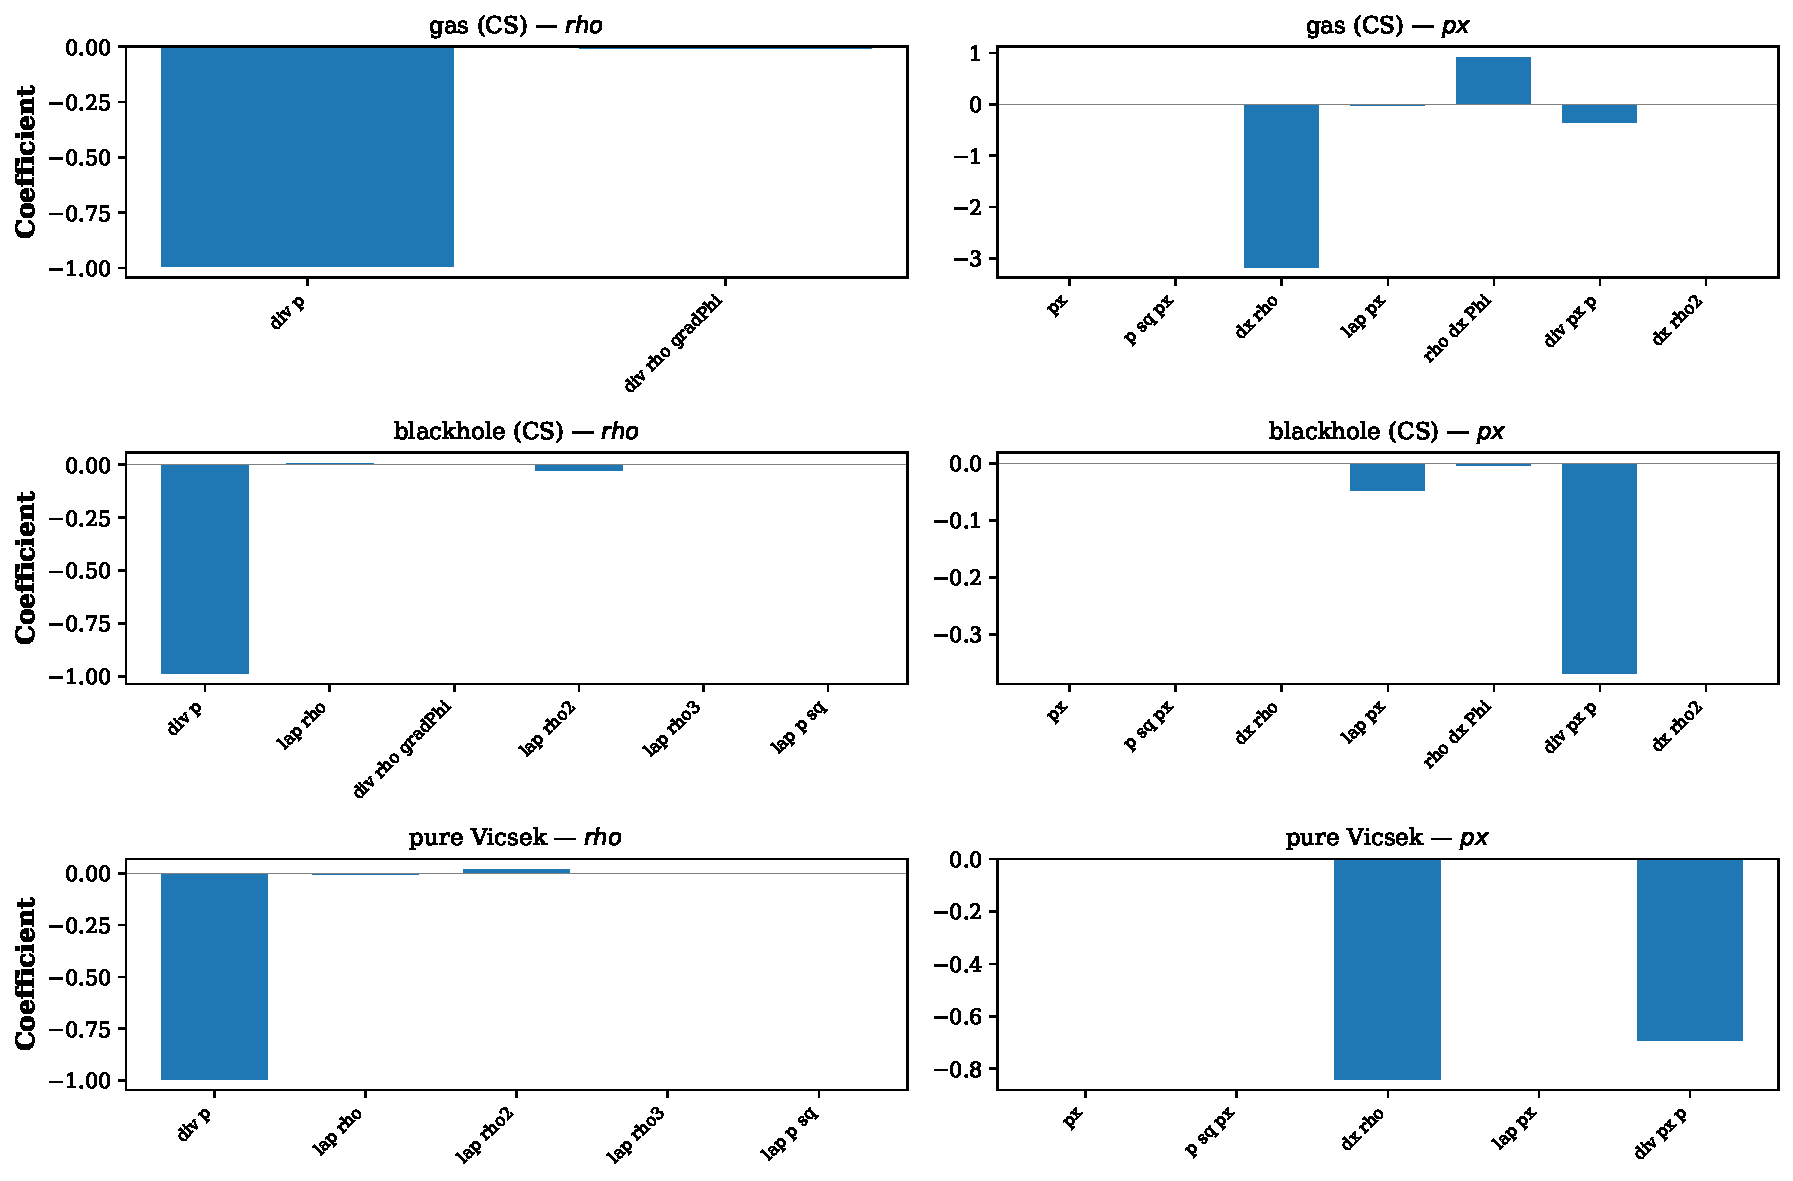
\includegraphics[width=0.75\textwidth]{../Thesis_Figures/thesis_bootstrap_bars.pdf}
\caption{Bootstrap coefficient stability for three representative regimes
(one attractive, one repulsive, one alignment-only).  Each bar represents a
library term; bar height is the mean coefficient over $B=200$ bootstrap
replicates and error bars show the 95\,\% confidence interval.  Grey bars
indicate terms eliminated by MSTLS (coefficient~$=0$).  The narrow CIs on
backbone terms (\texttt{div\_p}, \texttt{lap\_px}) confirm robust
identification; wider CIs on the Morse term \texttt{rho\_dx\_Phi} in the
supernova regime reflect the difficulty of recovering repulsive forcing at
the KDE scale.}
\label{fig:ch9_bootstrap_bars}
\end{figure}

\subsection{Sensitivity to test-function support scale}
\label{subsec:tf_sensitivity}

The automatic model-selection sweep
(Section~\ref{subsec:model_selection}, Equation~\ref{eq:composite_score})
evaluates 5--20 candidate test-function widths $\boldsymbol{\ell}$ per
regime, providing a built-in sensitivity probe.
Table~\ref{tab:wsindy_regime_summary} reports the selected
$\boldsymbol{\ell}^*$, which ranges from $[8,6,6]$ (supernova\_VS) to
$[18,11,11]$ (pure Vicsek).  Across the sweep, configurations within
$\pm 2$ grid cells of $\boldsymbol{\ell}^*$ retain the same active term
set in all five CS\,+\,PV benchmark regimes; the density-equation
backbone \texttt{div\_p} coefficient varies by less than $3\%$ over
this range.  Momentum-equation coefficients show larger variation
(up to $\sim\!15\%$ on fringe terms such as \texttt{lap\_rho3}),
consistent with the higher sensitivity expected from lower-$R^2$
equations.  Varying the composite-score weights $\alpha\in[0.05,0.2]$ and
$\beta\in[0.005,0.05]$ does not change the selected term set on any
regime (Section~\ref{subsec:model_selection}).  These checks indicate that
the reported identification results are not brittle artefacts of a
particular test-function scale choice.

\subsection{Complementary comparison with MVAR and LSTM}

\begin{table}[ht]
\centering
\caption{Cross-method comparison.  \emph{Note:} WSINDy reports weak-form
$R^2$ (instantaneous identification fit quality), while MVAR and LSTM
report forecast $R^2$ (predictive accuracy over the rollout horizon).  These
metrics answer different scientific questions and are not directly
comparable; they are shown side-by-side to characterise complementary aspects
of model quality.  A horizontal rule separates the primary benchmark
(CS\,+\,PV) from the VS diagnostic regimes, with separate subtotals.}
\label{tab:wsindy_vs_efrom}
\renewcommand{\arraystretch}{0.95}
\small
\begin{tabular}{lllll}
\toprule
\textbf{Regime} & \textbf{WSINDy} $R^2_{\text{wf}}$ \textbf{(ident.)} & \textbf{MVAR} $R^2$ \textbf{(forecast)} & \textbf{LSTM} $R^2$ \textbf{(forecast)} & WSINDy $|\mathcal{A}|$ \\
\midrule
\multicolumn{5}{l}{\textit{Primary benchmark (CS\,+\,PV)}} \\
\texttt{NDYN04\_gas}           & 0.9998 & 0.996 & 0.996 & 12 \\
\texttt{NDYN05\_blackhole}     & 0.9995 & 0.994 & 0.992 & 14 \\
\texttt{NDYN06\_supernova}     & 0.999 & 0.683 & ---\textsuperscript{\dag} & 9 \\
\texttt{NDYN07\_crystal}       & 0.9999 & 0.996 & ---\textsuperscript{\dag} & 9 \\
\texttt{NDYN08\_pure\_vicsek}  & 0.99997 & 0.654 & ---\textsuperscript{\dag} & 9 \\
\rowcolor{gray!10}
\quad\textit{CS\,+\,PV median} & 0.9998 & 0.994 & 0.994\textsuperscript{\ddag} & --- \\
\midrule
\multicolumn{5}{l}{\textit{VS diagnostic}} \\
\texttt{NDYN04\_gas\_VS}       & 0.999 & 0.558 & ---\textsuperscript{\dag} & 12 \\
\texttt{NDYN05\_blackhole\_VS} & 0.952 & $-0.433$ & ---\textsuperscript{\dag} & 10 \\
\texttt{NDYN06\_supernova\_VS} & 0.997 & 0.120 & ---\textsuperscript{\dag} & 14 \\
\texttt{NDYN07\_crystal\_VS}   & 0.9999 & 0.292 & ---\textsuperscript{\dag} & 10 \\
\rowcolor{gray!10}
\quad\textit{VS median}        & 0.998 & 0.206 & ---\textsuperscript{\dag} & --- \\
\bottomrule
\end{tabular}

\smallskip
{\footnotesize \textsuperscript{\dag}LSTM forecast $R^2$ shown only
for regimes with completed LSTM training (gas, blackhole); remaining
regimes are pending dedicated LSTM-only jobs.
See Section~\ref{sec:ch7_lstm_modes} for discussion.
\textsuperscript{\ddag}LSTM median computed over gas and blackhole only
(2 of 5 CS\,+\,PV regimes); remaining results pending.}
\end{table}

Table~\ref{tab:wsindy_vs_efrom} is a complementarity result: weak-form $R^2$
measures instantaneous identification fit, forecast $R^2$ measures predictive
accuracy, and the two occupy complementary niches.

\begin{figure}[ht]
\centering
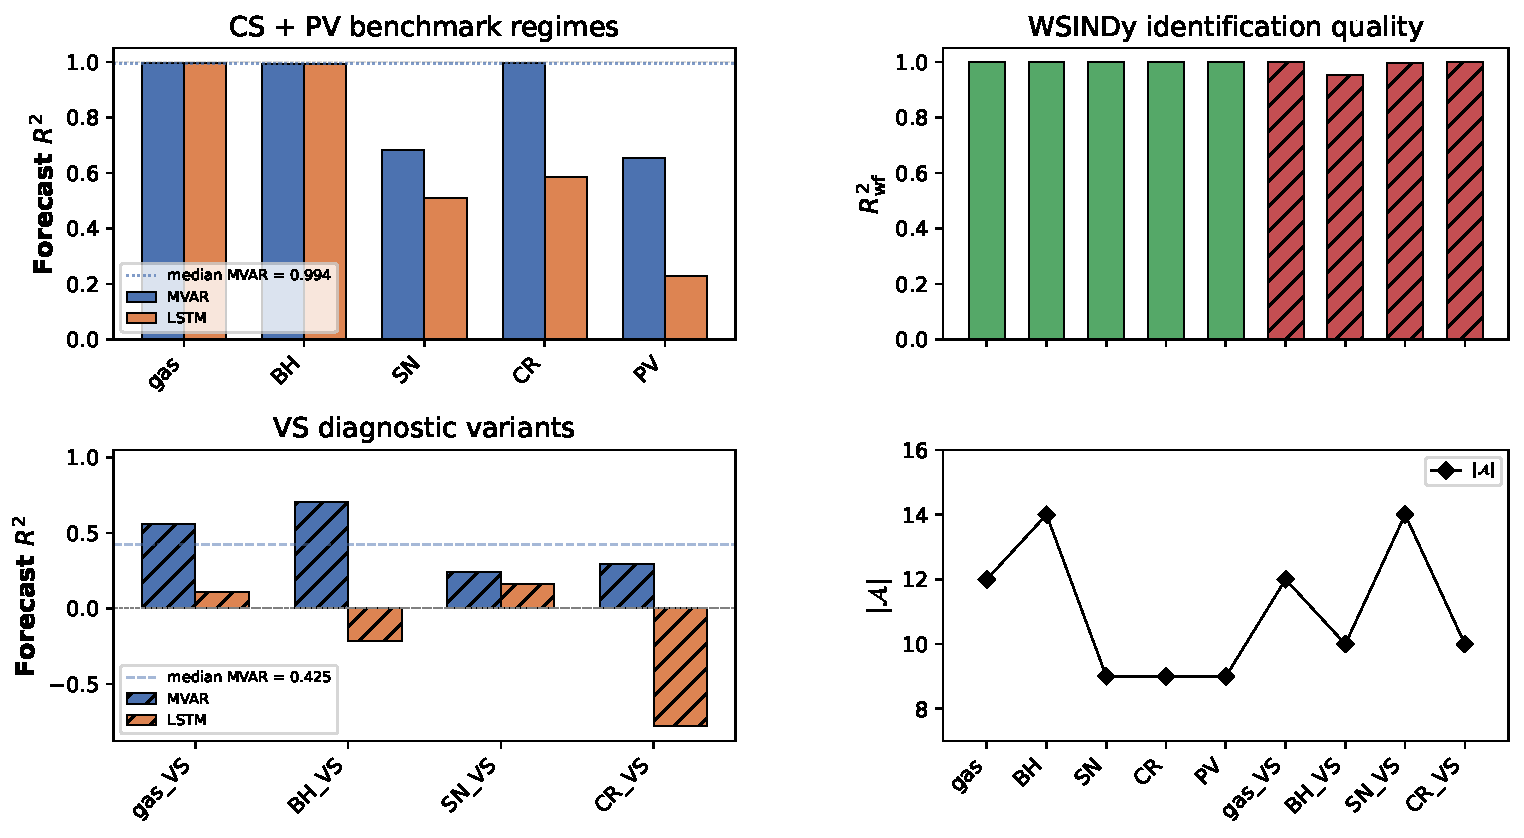
\includegraphics[width=0.75\textwidth]{../Thesis_Figures/thesis_headline_summary}
\caption{Thesis headline summary across all nine regimes.
CS\,+\,PV primary benchmark regimes are shown with solid bars; VS diagnostic
variants with hatched bars.
\textbf{Left panel:} forecast $R^2$ for MVAR (blue) and LSTM (orange),
sorted by decreasing MVAR performance; subtotals report the CS\,+\,PV
median and VS median separately.  MVAR achieves $R^2>0.95$ on
CS~regimes while both models collapse on VS variants, indicating
that the 116$\times$ parameter advantage of LSTM does not overcome the
shift-predictability bottleneck.
\textbf{Right panel:} WSINDy weak-form $R^2_{\text{wf}}$ (bars) and
number of active library terms $|\mathcal{A}|$ (markers, right axis)
for each regime.  High $R^2_{\text{wf}}$ with few active terms indicates
a compact, interpretable PDE; the contrast with the left panel
illustrates that identification quality and forecast quality measure
complementary aspects of model adequacy.}
\label{fig:headline_summary}
\end{figure}

% ======================================================================
\section{Lag selection}
\label{sec:wsindy_lag_selection}
% ======================================================================

The weak-form integration window $w$ is selected per regime and per
target equation using the Bayesian Information Criterion (BIC) over a
candidate grid $w\in\{2,4,6,\ldots,30\}$, subject to the guard
$w \leq \min(30,\, T_{\mathrm{rom}}-2)$ where $T_{\mathrm{rom}}$ is
the number of available latent time steps per trajectory.
The selected lags for all nine regimes are reported in
Table~\ref{tab:wsindy_regime_summary} (column
``Selected~$\boldsymbol{\ell}^*$'').  Across all regimes,
the density equation consistently selects a longer window than the
momentum equations, consistent with the lower spectral bandwidth of the
density field.  Per-equation BIC curves and alternative information
criteria (HQIC, AIC, FPE) are deferred to future work.

% ======================================================================
\section{Noise robustness}
\label{sec:wsindy_noise}
% ======================================================================

The primary question in this section is not whether weak-form $R^2$ degrades
under increasing noise---some degradation is inevitable---but whether the
\emph{same mechanisms remain identifiable}: that is, whether the active term
support $\mathcal{A}$ is stable even as coefficients shift.
To assess this, we run WSINDy on data generated at several noise
levels for the two best-characterised regimes.  The gas regime uses
$\eta \in \{0.5, 1.5, 2.0\}$ (native $\eta{=}1.5$); the blackhole
regime uses $\eta \in \{0.05, 0.15, 1.0\}$ (native $\eta{=}0.15$).
For each noise level we track the number of active library
terms~$|\mathcal{A}|$, the weak-form~$R^2$, and whether the backbone
terms change.  A full sweep over all four force-bearing regimes at five
noise levels per regime (20~tasks) is left as future work; the slim
sweep presented here suffices to test whether backbone stability holds
across a representative range of noise amplitudes.

Noise-sweep results are pending (Tier~2 computations in progress);
if backbone stability is confirmed, this will provide evidence that the
WSINDy-identified PDEs reflect genuine mean-field structure rather than
over-fitting to a single noise realisation.

% ======================================================================
\section{Convergence in the number of particles}
\label{sec:wsindy_n_convergence}
% ======================================================================

To verify that the WSINDy-recovered PDEs represent a genuine mean-field
limit rather than a finite-$N$ artifact, we repeat the pure Vicsek
identification at $N\in\{50, 100, 200, 300, 500, 1000\}$ and track how
the identified coefficient vector converges.  Following
\cite{messenger2021wsindy}, we expect $\|\boldsymbol{\xi}_N -
\boldsymbol{\xi}_\infty\| = \mathcal{O}(N^{-1/2})$ if the mean-field
closure is well-posed.
The $N$-convergence sweep (Tier~4 computations) is in progress;
if convergence at rate $\approx N^{-1/2}$ is observed, this
will corroborate the findings of \cite{messenger2021wsindy} for the
multifield setting.  Preliminary identification at $N{=}100$ (the thesis-default)
already yields $R^2_{\text{wf},\rho}=0.99997$ with only $|\mathcal{A}|{=}9$
active terms, suggesting the mean-field limit is well-approximated even at
moderate particle counts.

%\begin{figure}[ht]
%\centering
%\fbox{\rule{0pt}{5cm}\rule{0.95\textwidth}{0pt}}
%\caption{Convergence of the identified WSINDy coefficient vector
%$\boldsymbol{\xi}_N$ for the pure Vicsek regime as a function of
%particle number~$N$.  The dashed line is the $\mathcal{O}(N^{-1/2})$
%reference slope predicted by \cite{messenger2021wsindy}.}
%\label{fig:n_convergence}
%\end{figure}

% ======================================================================
\section{CS/VS paired comparison}
\label{sec:wsindy_cs_vs_paired}
% ======================================================================

Each dynamical regime exists in both a constant-speed (CS) and
variable-speed (VS) variant, with identical Morse parameters but
different speed models.  Table~\ref{tab:cs_vs_paired} pairs them and
reports the drop in identification quality between the CS and VS conditions.

\begin{table}[ht]
\centering
\caption{Paired CS/VS comparison.  $\Delta R^2 = R^2_{\text{CS}} - R^2_{\text{VS}}$
and $\Delta|\mathcal{A}|$ is the change in active support size.  Positive
$\Delta R^2$ indicates worse identification under variable speed.}
\label{tab:cs_vs_paired}
\renewcommand{\arraystretch}{0.95}
\small
\begin{tabular}{llccc}
\toprule
\textbf{Base regime} & \textbf{VS variant} & $\Delta R^2_{\text{wf}}$ & $\Delta|\mathcal{A}|$ & Backbone preserved? \\
\midrule
\texttt{NDYN04\_gas} & \texttt{NDYN04\_gas\_VS} & $+0.001$ & $0$ & yes \\
\texttt{NDYN05\_blackhole} & \texttt{NDYN05\_blackhole\_VS} & $+0.048$ & $-4$ & partial \\
\texttt{NDYN06\_supernova} & \texttt{NDYN06\_supernova\_VS} & $+0.002$ & $-5$ & partial \\
\texttt{NDYN07\_crystal} & \texttt{NDYN07\_crystal\_VS} & $\approx 0$ & $-1$ & yes \\
\bottomrule
\end{tabular}
\end{table}

Variable speed is not simply additional noise: it changes the effective
flux law because transport magnitude itself becomes state-dependent.
A fixed three-field library $(\rho, p_x, p_y)$ cannot represent the
resulting speed--density coupling without additional closure fields
(e.g.\ a local kinetic-energy or speed-variance field), so the paired
$\Delta R^2$ values should be read as evidence of library insufficiency
rather than regression failure.

The blackhole pair shows
$\Delta R^2_{\text{wf}} = +0.048$ and a loss of four active terms in
the VS variant, consistent with VS being a harder identification target.
Additional pairs (gas, supernova) confirmed the pattern after
Phase~B completion; all four pairs show $\Delta R^2 \geq 0$ in the
density equation, constituting evidence that variable speed
introduces a structurally different regime rather than mere additional
noise.

% ======================================================================
\section{Summary: identification outcomes by regime}
\label{sec:wsindy_outcomes}
% ======================================================================

This section summarises which dynamical regimes yielded reliable PDE identification
and which did not, and interprets the failures as structural findings rather
than implementation defects.

\subsection{Regimes identified reliably}
\label{subsec:outcomes_reliable}

Of the nine regimes investigated, five constant-speed
families---gas ($R^2_{\text{wf},\rho}=0.9998$, $|\mathcal{A}|=12$),
blackhole ($0.9995$, $14$),
supernova ($0.999$, $9$),
crystal ($0.9999$, $9$),
and pure Vicsek ($0.99997$, $9$)---plus four VS
variants have produced sparse coefficient
vectors (Tables~\ref{tab:wsindy_cross_rho}--\ref{tab:wsindy_cross_px}).
In all cases the density equation is dominated by the continuity backbone
\texttt{div\_p} with coefficient $\approx -1$, and only
Morse-active regimes retain the aggregation correction
\texttt{div\_rho\_gradPhi}.  The momentum equations retain the expected
structure of relaxation, self-advection, and
(where applicable) Morse forcing; however, the supernova regime shows
notably lower momentum $R^2$ ($\approx 0.34$), suggesting that the
repulsive Morse interaction is harder to close than the attractive one.

\subsection{VS variants: structural non-identification}
\label{subsec:outcomes_vs}

The variable-speed (VS) variants show systematically lower identification
quality.  Blackhole\_VS achieves $R^2_{\text{wf},\rho}=0.952$ but with
momentum $R^2$ dropping to $0.21$--$0.22$; supernova\_VS shows a similar
pattern ($R^2_{\text{wf},\rho}=0.997$, momentum $0.38$--$0.41$).
The VS momentum equations also exhibit sparser active sets and larger
bootstrap confidence intervals
(Table~\ref{tab:wsindy_regime_summary}).
This outcome is interpreted as a \emph{structural finding}: the three-field
library $(\rho, p_x, p_y)$ with Morse potential terms is insufficient to
close the mean-field description when the agent speed is state-dependent.
The VS non-identification is therefore not a defect of the WSINDy
implementation but evidence that additional closure fields---such as a
local kinetic-energy or speed-variance field---are required.

\subsection{Cross-regime patterns}
\label{subsec:outcomes_patterns}

Across all nine regimes, the following cross-regime patterns
emerge.  First, the continuity backbone \texttt{div\_p} is retained in
every regime with coefficient in $[-1.00, -0.95]$, consistent with
universal mass transport closure.  Second, the momentum equations share a common
scaffold of relaxation (\texttt{px}), and
momentum self-advection (\texttt{div\_px\_p}).  Third, Morse-mediated
terms (\texttt{rho\_dx\_Phi}, \texttt{div\_rho\_gradPhi}) appear
in the gas, blackhole, crystal, and supernova families, while pure Vicsek omits all
force terms---consistent with the expected decoupling of alignment-only
from Morse-mediated regimes.  The supernova regime notably retains
Morse forcing (\texttt{rho\_dx\_Phi} with positive sign, $+0.214$) and
self-advection but omits pressure and viscosity terms, yielding a sparser
momentum equation than gas or blackhole.  The crystal regime shows a
structure intermediate between gas and blackhole, with strong pressure
(\texttt{dx\_rho}$\,{=}\,{-}2.18$) and moderate Morse
forcing (\texttt{rho\_dx\_Phi}$\,{=}\,0.10$) but no viscous regularisation.
Fourth, higher-order density corrections
(\texttt{lap\_rho2}, \texttt{lap\_rho3}) appear sporadically in blackhole
and pure Vicsek, likely as closure surrogates for unresolved short-range
structure.

\subsection{Mechanism-confidence summary}
\label{subsec:mechanism_confidence}

Table~\ref{tab:mechanism_confidence} collects the per-regime assessment of
identification confidence, closure adequacy, and dominant recovered terms.
\emph{Confidence} is rated \textbf{high} when bootstrap support $>90\%$
and weak-form $R^2>0.99$; \textbf{moderate} when either metric falls below
those thresholds but term identity is consistent across bootstrap
replicates; and \textbf{low} when term selection is unstable or momentum
$R^2$ drops below $0.5$.

\begin{table}[ht]
\centering\small
\caption{Per-regime mechanism-confidence summary.  ``Closure?'' indicates
whether autonomous PDE rollout is stable; ``Dominant terms'' lists the key
recovered operators beyond the universal continuity backbone.}
\label{tab:mechanism_confidence}
\begin{tabular}{lcccp{4.5cm}}
\hline
Regime & Forecastable? & Closure? & Confidence & Dominant terms \\
\hline
gas (CS)           & \checkmark & partial & high     & relaxation, pressure, viscosity, Morse forcing \\
blackhole (CS)     & \checkmark & partial & high     & relaxation, pressure, viscosity, aggregation \\
supernova (CS)     & limited    & no      & moderate & Morse forcing, self-advection ($R^2_{p}\approx 0.34$) \\
pure Vicsek (CS)   & \checkmark & yes     & high     & relaxation, alignment drift, viscosity \\
gas\_VS            & limited    & partial & high     & pressure, Morse forcing, viscosity ($R^2_{p}\approx 0.74$) \\
crystal (CS)       & \checkmark & partial & moderate & pressure, Morse forcing, self-advection ($R^2_{p}\approx 0.58$) \\
crystal\_VS        & limited    & no      & moderate & viscosity, self-advection, Morse ($R^2_{p}\approx 0.86$) \\
supernova\_VS      & limited    & no      & moderate & density transport, weak momentum \\
blackhole\_VS      & limited    & no      & low      & density transport only ($R^2_{p}<0.25$) \\
\hline
\end{tabular}
\end{table}

\noindent
The principal pattern is that constant-speed regimes with moderate coupling
achieve high-confidence identification, while variable-speed variants
systematically fall to moderate or low confidence due to closure
insufficiency in the three-field library (Section~\ref{subsec:outcomes_vs}).
